%%%%%
%%%%%  Use LUALATEX, not LATEX.
%%%%%
%%%%
\documentclass[]{VUMIFTemplateClass}

\usepackage{indentfirst}
\usepackage{amsmath, amsthm, amssymb, amsfonts}
\usepackage{mathtools}
\usepackage{physics}
\usepackage{graphicx}
\usepackage{verbatim}
\usepackage[hidelinks]{hyperref}
\usepackage{xcolor,algorithm,algorithmic}
\definecolor{gray}{gray}{0.6}


\usepackage{tcolorbox}

\newcommand{\yellowcomment}[1]{%
    \begin{tcolorbox}[colback=yellow!80, colframe=yellow!80, arc=0pt, outer arc=0pt, boxrule=0pt, left=3pt, right=3pt, top=3pt, bottom=3pt]
        \textbf{\textcolor{red}{COMMENT:}} #1
    \end{tcolorbox}
}

\newcommand{\warningcomment}[1]{%
    \begin{tcolorbox}[colback=yellow!90, colframe=red, arc=0pt, outer arc=0pt, boxrule=2pt, left=5pt, right=5pt, top=5pt, bottom=5pt]
        \Large\textbf{\textcolor{red}{FIX THIS: }} \normalsize #1
    \end{tcolorbox}
}

\newcommand{\goodcomment}[1]{%
    \begin{tcolorbox}[colback=green!20, colframe=green!60, arc=0pt, outer arc=0pt, boxrule=1pt, left=3pt, right=3pt, top=3pt, bottom=3pt]
        \textbf{\textcolor{green!70!black}{GOOD:}} #1
    \end{tcolorbox}
}

\newcommand{\noticecomment}[1]{%
    \begin{tcolorbox}[colback=blue!20, colframe=blue!60, arc=0pt, outer arc=0pt, boxrule=1pt, left=3pt, right=3pt, top=3pt, bottom=3pt]
        \textbf{\textcolor{blue!70!black}{NOTE:}} #1
    \end{tcolorbox}
}

\newcommand{\todocomment}[1]{%
    \begin{tcolorbox}[colback=red!20, colframe=red!60, arc=0pt, outer arc=0pt, boxrule=1pt, left=3pt, right=3pt, top=3pt, bottom=3pt]
        \textbf{\textcolor{orange!70!black}{TODO:}} #1
    \end{tcolorbox}
}

\newcommand{\suggestioncomment}[1]{%
    \definecolor{lime}{RGB}{50,205,50}%
    \begin{tcolorbox}[colback=lime!15, colframe=lime!60, arc=0pt, outer arc=0pt, boxrule=1pt, left=3pt, right=3pt, top=3pt, bottom=3pt]
        \textbf{\textcolor{lime!70!black}{SUGGESTION:}} #1
    \end{tcolorbox}%
}



\newenvironment{mpitemlist}[1][\linewidth]{%
    \begin{minipage}[t]{#1}%
        \setlength{\leftmargini}{12pt}%
        \begin{itemize}%
            \setlength{\itemsep}{1pt}%
            \setlength{\parskip}{0pt}%
            \setlength{\parsep}{0pt}%
}{%
        \end{itemize}%
    \end{minipage}\newline
}

\usepackage[nottoc]{tocbibind}
\usepackage{tocloft}
\usepackage{longtable}
\usepackage{amssymb}

\usepackage{titlesec}
\newcommand{\sectionbreak}{\clearpage}

\makeatletter
\renewcommand{\fnum@algorithm}{\thealgorithm}
\makeatother
\renewcommand\thealgorithm{\arabic{algorithm} algorithm}

\usepackage{biblatex}
\bibliography{bibliografija}
%% to change the numbering (numeric or alphabetic) of bibliographic sources, make the change in VUMIFTemplateClass.cls, line 139

% Author's MACROS
\newcommand{\EE}{\mathbb{E}\,} % Mean
\newcommand{\ee}{{\mathrm e}}  % nice exponent
\newcommand{\RR}{\mathbb{R}}

\makeatletter
% introduce a 4th-level sectioning command: \subsubsubsection
\newcounter{subsubsubsection}[subsubsection]
\renewcommand\thesubsubsubsection{\thesubsubsection.\arabic{subsubsubsection}}

\providecommand\subsubsubsection{%
    \@startsection{subsubsubsection}{4}{\z@}%
        {-3.25ex\@plus -1ex \@minus -.2ex}%
        {1.5ex \@plus .2ex}%
        {\normalfont\normalsize\bfseries}%
}

% ensure numbering and TOC include this level
\setcounter{secnumdepth}{4}
\setcounter{tocdepth}{4}
\makeatother


\studyprogramme{Software Engineering} %Write your study programme (example – Software engineering, Financial and Actuarial Mathematics, etc.)
\worktype{PS Software Design} % Bachelor's thesis or Master's thesis
\worktitle{PS Sofware Design documentation}
% \secondworktitle{Work Title in Lithuanian}
\workauthor{Tadas Riksas, Darius Spruogis, Gustas Mickus, Julius Jauga}

%There may be more than one author, in which case each author is written from a new line which is added in Titlepage.tex or LongerTitlePage.tex
%\secondauthor{Name Surname} %If present, otherwise delete

\supervisor{Vasilij Savin}
% \reviewer{pedagogical/scientific title Name Surname} %If present, otherwise delete
% \scientificadvisor{pedagogical/scientific title Name Surname} %If present, otherwise delete

\begin{document}
\selectlanguage{english}

\onehalfspacing
\begin{titlepage}
\vskip 20pt
\begin{center}

\includegraphics[scale=0.55]{images/MIF.png}
\end{center}

\makeatletter

\vskip 20pt
\centerline{\bf \large \textbf{VILNIUS UNIVERSITY}}
\vskip 10pt
\centerline{\large \textbf{FACULTY OF MATHEMATICS AND INFORMATICS}}
\vskip 10pt
\centerline{\large \textbf{\MakeUppercase{\@studyprogramme \space study programme}}}

\vskip 80pt
\centerline{\Large \@worktype}
\vskip 20pt
\begin{center}
    {\bf \LARGE \@worktitle}
\end{center}
\begin{center}
    {\bf \Large \@secondworktitle}
\end{center}
\vskip 80pt

\centering{\Large \@workauthor}
\@ifundefined{@secondauthor}{}
{
\vskip 10pt
\centering{\Large \@secondauthor}
}
\vskip 20pt

\centering{
    \begin{tabular}{rcp{.7\textwidth}}
        {\Large Supervisor} & {\Large :} & {\Large \@supervisor}\\[10pt]
        \@ifundefined{@scientificadvisor}{}
            {
                {\Large Scientific advisor} & {\Large :} & {\Large \@scientificadvisor}\\[10pt]
            }
        \@ifundefined{@reviewer}{}
            {
                {\Large Reviewer} & {\Large :} & {\Large \@reviewer}\\[10pt]
            }
    \end{tabular}}


\vskip 110pt

\centerline{\large \textbf{Vilnius}}
\centerline{\large \textbf{\the\year{}}}

\makeatother

\newpage
\end{titlepage}
%\newgeometry{top=2cm,bottom=2cm,right=2cm,left=3cm}
\setcounter{page}{2}


\tableofcontents
\onehalfspacing


\warningcomment{
\begin{itemize}
    \item mazinkit teksto kieki, pagalvokit ar patys turedami sia dokumentacija skaitytumete ta visa teksta
    \item diagramose nevaizduojame sistemos vidaus
    \item visi flows turi BUTI paremti grafine sasaja, jeigu to nera tai labai sunku isitikinti ar business flows nesusikerta su kita sistemos logika
    \item Duomenu modeliui aprasyti naudokite latex lenteles, ne teksta, teksta sunku skaityti.
    \item duomenu modelis turi buti pagristas business flowsais ar GUI pavydziais.
    \item reiketu apriboti dokumento ilgi, nuspresti kiek.
\end{itemize}
}

\warningcomment{Nenaudoti chatgpt, tekstas gaunasi nuobodus, atsiranda daug faktiniu klaidu}

\noticecomment{dokumento struktura: sections 1,2,3 naudojame isskaidyti funkcionalumo sritis (pvz orders, serving, login, management), subsection naudojame pazymeti GUI, business flows, package diagrams, data model, api contract.}


\section*{Introduction}
This document focuses on what kind of software is needed for order and appointment based businesses to manage their operations without any hiccups.

The structure of the document is:
\begin{itemize}
    \item Introduciton
    \item Functionallity \begin{itemize}
        \item GUI
        \item Business flow(s)
        \item Package diagram(s)
        \item Data model    
    \end{itemize}
    \item API Contracts
    \item Conclusion
\end{itemize}

Note: after making 80+ Figma GUI wire-frames we realized that there is really no limit to the domain size of this application. While we did cover all the essential functionality, there is still a lot of questions left to solve. Here are some of them that we encountered:
\begin{itemize}
    \item How product supply chains work? How our system integrates that? (For inventory management)
    \item What to do in case payment system (Stripe) goes down? How will the system manage that?
    \item etc.
\end{itemize}
And there are way way more things to take in consideration! But writing all these things out would make this document huge and unreadable. Highlighting this problem we want to show not that this document lacks some features (or to put simply sucks) but that simply the design of these systems goes way beyond the scope of what we can capture in this course. Therefore we will limit ourselves mostly to those 80+ GUIs that we made, especially focusing on the GUIs that feature creating and updating forms.

While making the GUIs we also noticed that in the future the client could always require more features to be added such as:
\begin{itemize}
    \item LLM chat support
    \item etc.
\end{itemize}
As a result, we will try to make the system as future proof as possible.

So why so many GUIs wire-frames? After trying to write this document for the first time using only text for describing how users interact with the system we kind of failed. After that failure we decided that it would be ideal to simply use Figma and quickly prototype as much GUIs as possible for all features. This would allow each team member quickly to understand how their colleges understand the business problem and if there are any problems with that understanding. It also served as a great way to ensure consistency between system components. We hope that the reader will appreciate our huge effort put into these GUIs and that their job will be easier.

\section*{Important links}
Before you start it would be ideal if you familiarized your self with GUIs. This will help you to better understand the workings of the system, what data is passed around and how users interact with our system.

You can use the link below to explore the prototypes in Figma, just simply click anywhere and Figma will show you what buttons and navigation links are clickable with pulsing animation.

\href{https://www.figma.com/design/IpiyOU6rDdMWJAuKfbXnuQ/HCI-2025-mockups?node-id=0-1&t=qFGqf8yRbP1gP6IJ-1}{Figma prototypes}




\section{Functionality}
We will discuss here the GUIs of the application, business flows, package diagrams and data model.

\subsection{Order Management (Bars/Restaurants)}


\noticecomment{Client order = seating + placing menu items + payment}

\noticecomment{In a real system, you might need to consider how orders are communicated (e.g., a screen in the kitchen, notifications), but this is left as a design decision for the team.}

\begin{longtable}{p{0.25\linewidth} p{0.70\linewidth}}
\caption{Use cases for the Order Management domain} \\
\textbf{Use case} & \textbf{Description} \\
\hline
\endfirsthead

\multicolumn{2}{c}{{\tablename\ \thetable{} -- Continued from previous page}} \\
\textbf{Use case} & \textbf{Description} \\
\hline
\endhead

\multicolumn{2}{c}{{Continued on next page}} \\
\endfoot

\endlastfoot

Client Seating (Available) &
\begin{minipage}[t]{\linewidth}
Employee checks seating via POS. If available, employee assigns a table and confirms with client.
\end{minipage} \\[6pt]
\multicolumn{2}{@{}c@{}}{\color{gray}\rule{0.95\linewidth}{0.4pt}} \\[6pt]

Client Seating (Not Available) &
\begin{minipage}[t]{\linewidth}
Employee checks seating via POS, finds no seats available, and informs client.
\end{minipage} \\[6pt]
\multicolumn{2}{@{}c@{}}{\color{gray}\rule{0.95\linewidth}{0.4pt}} \\[6pt]

Place Order &
\begin{minipage}[t]{\linewidth}
Client requests menu, places an order via employee. If order is valid, client confirms, else corrections are requested.
\end{minipage} \\[6pt]
\multicolumn{2}{@{}c@{}}{\color{gray}\rule{0.95\linewidth}{0.4pt}} \\[6pt]

Modify Order &
\begin{minipage}[t]{\linewidth}
Client requests to update an existing order. Employee updates through POS, backend validates. On success, order is updated; on failure, errors are shown for correction.
\end{minipage} \\[6pt]
\multicolumn{2}{@{}c@{}}{\color{gray}\rule{0.95\linewidth}{0.4pt}} \\[6pt]

Cancel Order &
\begin{minipage}[t]{\linewidth}
Client requests to cancel an existing not completed order. Employee cancels through POS, backend validates that it is not completed. On success, order is updated; on failure, errors are shown.
\end{minipage} \\[6pt]
\multicolumn{2}{@{}c@{}}{\color{gray}\rule{0.95\linewidth}{0.4pt}} \\[6pt]

Mark items as delivered for table &
\begin{minipage}[t]{\linewidth}
The employee selects a table. The order with items are retrieved for that table, which is then displayed in the POS. The employee selects items to mark as delivered. The item status is updated in the backend server, and a confirmation is displayed in the POS.
\end{minipage} \\[6pt]
\multicolumn{2}{@{}c@{}}{\color{gray}\rule{0.95\linewidth}{0.4pt}} \\[6pt]

\end{longtable}

\subsubsection{Order client seating (available)}


\begin{figure}[H]
    \centering
    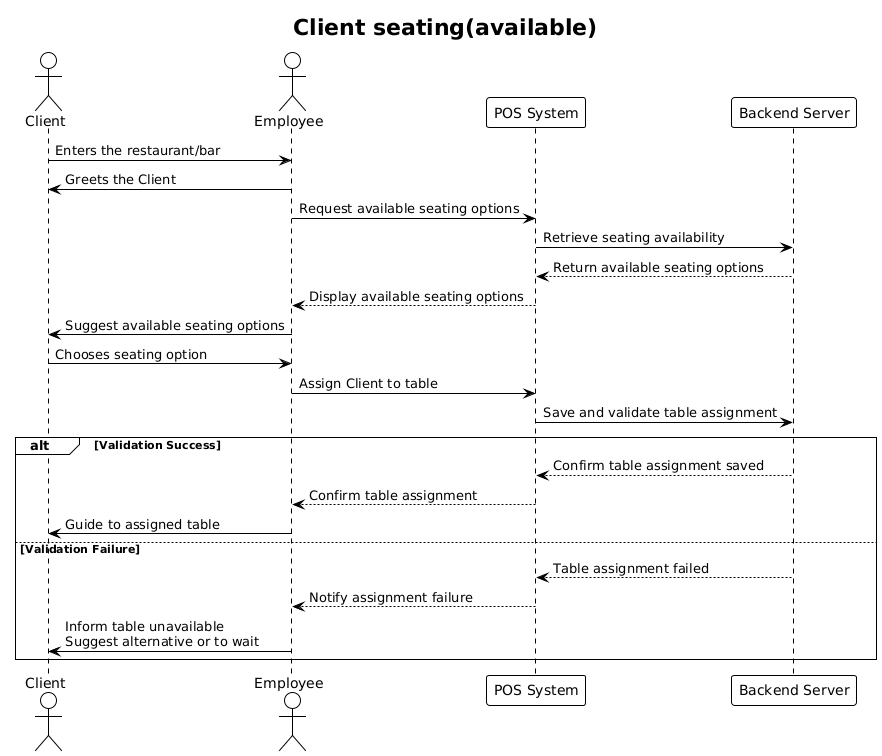
\includegraphics[width=0.8\textwidth]{images/diagrams/orders/order_client_seating_available.png}
    \caption{Client Seating(available) Sequence Diagram}
    \label{fig:client_seating_available_sequence}
\end{figure}

\subsubsection{Order client seating (not available) business flow}

\begin{figure}[H]
    \centering
    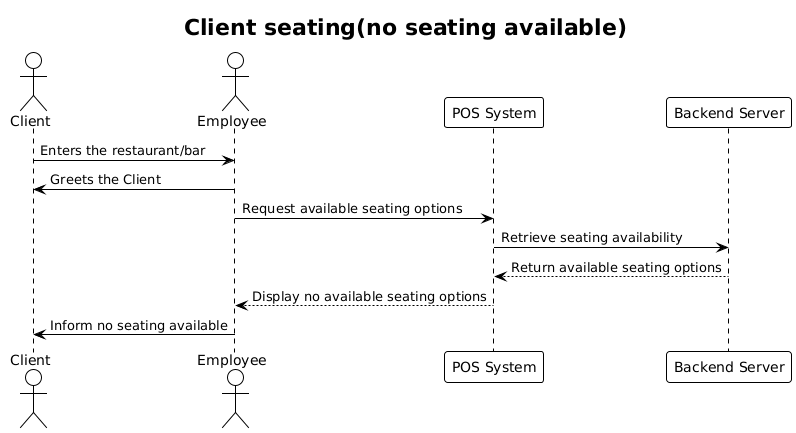
\includegraphics[width=0.8\textwidth]{images/diagrams/orders/order_client_seating_not_available_sequence.png}
    \caption{Client Seating(not available) Sequence Diagram}
    \label{fig:client_seating_not_available_sequence}
\end{figure}

\subsubsection{Place Order Business Flow}

\begin{figure}[H]
    \centering
    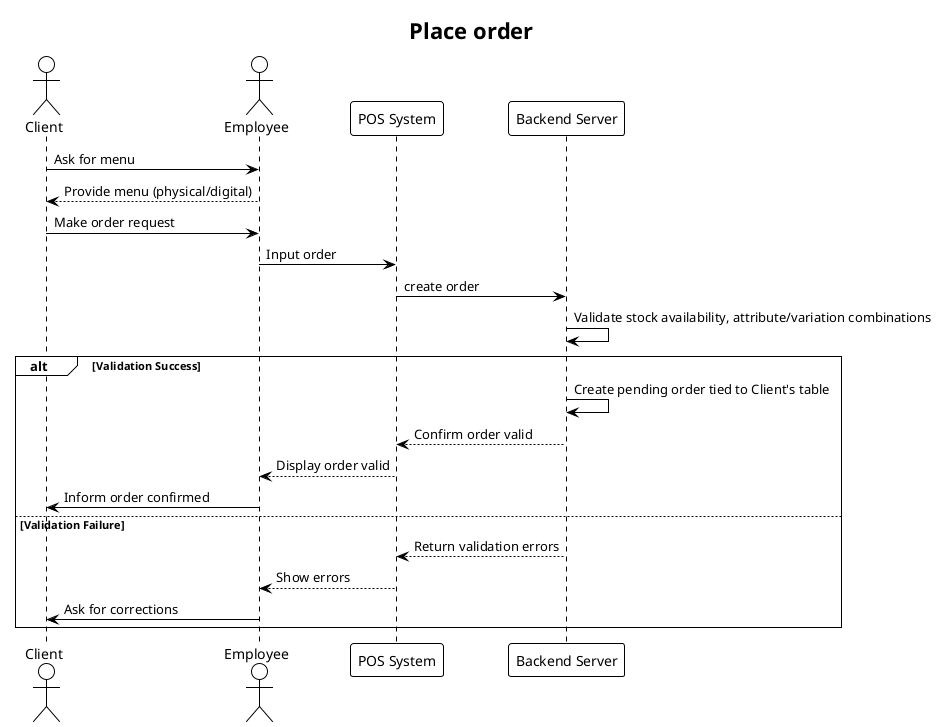
\includegraphics[width=0.8\textwidth]{images/diagrams/orders/order_place_order_sequence.png}
    \caption{Place Order Sequence Diagram}
    \label{fig:place_order_sequence}
\end{figure}

\subsubsection{Update Order Business Flow}


\begin{figure}[H]
    \centering
    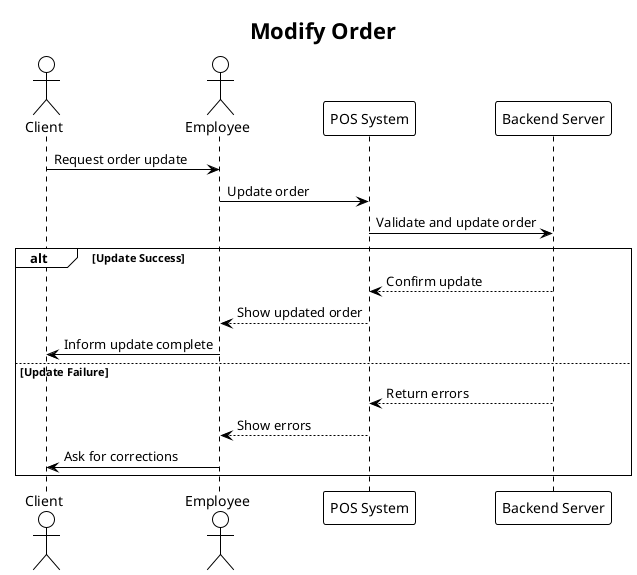
\includegraphics[width=0.8\textwidth]{images/diagrams/orders/order_modify_order_sequence.png}
    \caption{Modify Order Sequence Diagram}
    \label{fig:modify_order_sequence}
\end{figure}

\subsubsection{Order Cancellation Business Flow}


\begin{figure}[H]
    \centering
    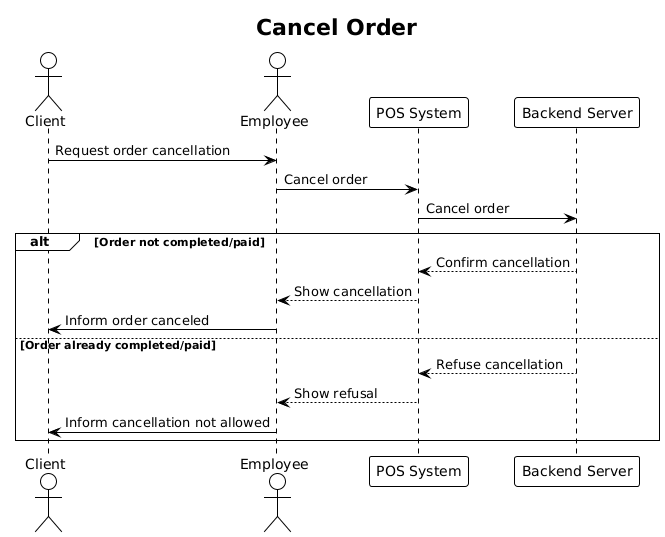
\includegraphics[width=0.8\textwidth]{images/diagrams/orders/order_cancel_order_sequence.png}
    \caption{Cancel Order Sequence Diagram}
    \label{fig:cancel_order_sequence}
\end{figure}

\subsubsection{Mark Items as Delivered for Table Business Flow}


\begin{figure}[H]
    \centering
    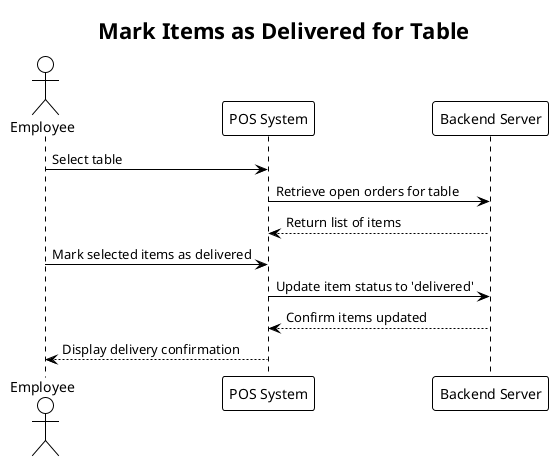
\includegraphics[width=0.8\textwidth]{images/diagrams/orders/order_mark_table_items_delivered_sequence.png}
    \caption{Mark Items as Delivered Sequence Diagram}
    \label{fig:mark_items_delivered_sequence}                   
\end{figure}


\subsection{Services Management (Spas/Salons)}

% ------------------------------------------------------------------------------
% Service Domain
% (Related to appointment-based businesses like spas, barbers, massage centers)
%
% Use Case             | Description
% ---------------------|-----------------------------------------------------------------
% Create Appointment   | Employee schedules a service for a customer (date, time, employee).
% Modify Appointment   | Change time, employee, service, date, or assigned employee.
% Cancel Appointment   | Cancel a scheduled service.
% Check Availability   | Verify if an employee is free at a given time.
% Send SMS Reminder    | Automatically send an SMS to the customer before the appointment.
% Assign Employee      | Assign a specialist to a service.
% Mark Service as Done | Record that the service has been completed.
% ------------------------------------------------------------------------------
\noticecomment{Dont forget SMS messages}

\noticecomment{The employee that registers the customer doesnt necessarily need to service the customer themselves (think of spas). However smaller businesses (like haircut saloons) employees may both register and service the customer themselves.}

We have identified the following use cases for the services management domain:

\vspace{1cm}
\begin{longtable}{p{0.25\linewidth} p{0.70\linewidth}}
\caption{Use cases for the Services Management domain} \\
\textbf{Use case} & \textbf{Description} \\
\hline
\endfirsthead

\multicolumn{2}{c}{{\tablename\ \thetable{} -- Continued from previous page}} \\
\textbf{Use case} & \textbf{Description} \\
\hline
\endhead

\multicolumn{2}{c}{{Continued on next page}} \\
\endfoot

\endlastfoot

Create appointment &
\begin{minipage}[t]{\linewidth}
Employee or customer schedules a service for a customer by selecting service, date/time and (optionally) employee; system reserves the slot, records booking metadata and sends confirmation.
\end{minipage} \\[6pt]
\multicolumn{2}{@{}c@{}}{\color{gray}\rule{0.95\linewidth}{0.4pt}} \\[6pt]

Modify appointment &
\begin{minipage}[t]{\linewidth}
Change appointment details (time, service, date, assigned employee); system validates availability, preserves historical record of changes and notifies affected parties.
\end{minipage} \\[6pt]
\multicolumn{2}{@{}c@{}}{\color{gray}\rule{0.95\linewidth}{0.4pt}} \\[6pt]

Cancel appointment &
\begin{minipage}[t]{\linewidth}
Customer or staff cancels an appointment; system frees the slot, applies cancellation rules (refund/deposit handling if applicable) and sends notifications.
\end{minipage} \\[6pt]
\multicolumn{2}{@{}c@{}}{\color{gray}\rule{0.95\linewidth}{0.4pt}} \\[6pt]

Service Customer &
\begin{minipage}[t]{\linewidth}
    The customer gets the service done by the assigned employee; employee marks the service as completed in the system, which updates records and triggers any follow-up actions (e.g., feedback request, payment processing).
\end{minipage} \\
\end{longtable}

\vspace{1cm}


\subsubsection{Appointment creating business flow}



\begin{center}
\setlength{\tabcolsep}{8pt}
\begin{tabular}{|p{0.48\linewidth}|p{0.48\linewidth}|}
\hline
\textbf{Tables/Entities} \newline
\begin{mpitemlist}

\end{mpitemlist}
&
\textbf{Components} \newline
\begin{mpitemlist}

\end{mpitemlist}
\\ \hline
\textbf{Actions} \newline
\begin{mpitemlist}

\end{mpitemlist}
&

\\ \hline
\end{tabular}
\end{center}


\subsubsection{Appointment modification business flow}




\begin{center}
\setlength{\tabcolsep}{8pt}
\begin{tabular}{|p{0.48\linewidth}|p{0.48\linewidth}|}
\hline
\textbf{Tables/Entities} \newline
\begin{mpitemlist}

\end{mpitemlist}
&
\textbf{Components} \newline
\begin{mpitemlist}

\end{mpitemlist}
\\ \hline
\textbf{Actions} \newline
\begin{mpitemlist}

\end{mpitemlist}
&

\\ \hline
\end{tabular}
\end{center}



\subsubsection{Cancel appointment business flow}


\begin{center}
\setlength{\tabcolsep}{8pt}
\begin{tabular}{|p{0.48\linewidth}|p{0.48\linewidth}|}
\hline
\textbf{Tables/Entities} \newline
\begin{mpitemlist}

\end{mpitemlist}
&
\textbf{Components} \newline
\begin{mpitemlist}

\end{mpitemlist}
\\ \hline
\textbf{Actions} \newline
\begin{mpitemlist}

\end{mpitemlist}
&

\\ \hline
\end{tabular}
\end{center}




\subsubsection{Service customer business flow}


\begin{center}
\setlength{\tabcolsep}{8pt}
\begin{tabular}{|p{0.48\linewidth}|p{0.48\linewidth}|}
\hline
\textbf{Tables/Entities} \newline
\begin{mpitemlist}

\end{mpitemlist}
&
\textbf{Components} \newline
\begin{mpitemlist}

\end{mpitemlist}
\\ \hline
\textbf{Actions} \newline
\begin{mpitemlist}

\end{mpitemlist}
&

\\ \hline
\end{tabular}
\end{center}





% ------------------------------------------------------------------------
% PAYMENT STUFF
% ------------------------------------------------------------------------


\subsection{Payment}

\subsubsection{Supported Payment Methods}
\begin{itemize}
\item Cash
\item Gift card
\item Credit/debit card (via Stripe)
\end{itemize}

\subsubsection{Key Business Rules}
\begin{itemize}
\item Split payments are supported: an order total can be paid by multiple parties and/or multiple payment methods.
\item Employees can add tips and apply discounts during payment.
\item Final receipts must include applicable taxes, tips, and discounts for each payment.
\item Closed/paid orders are preserved for audit purposes and can be refunded (partial or total).
\item Refund for card payments is processed through Stripe. For other methods, the status is updated in the system.
\end{itemize}

\subsubsection{Payment Flow}
The following sequence diagram illustrates the payment process, including split payments, tips, and refunds.

\begin{figure}[H]
    \centering
    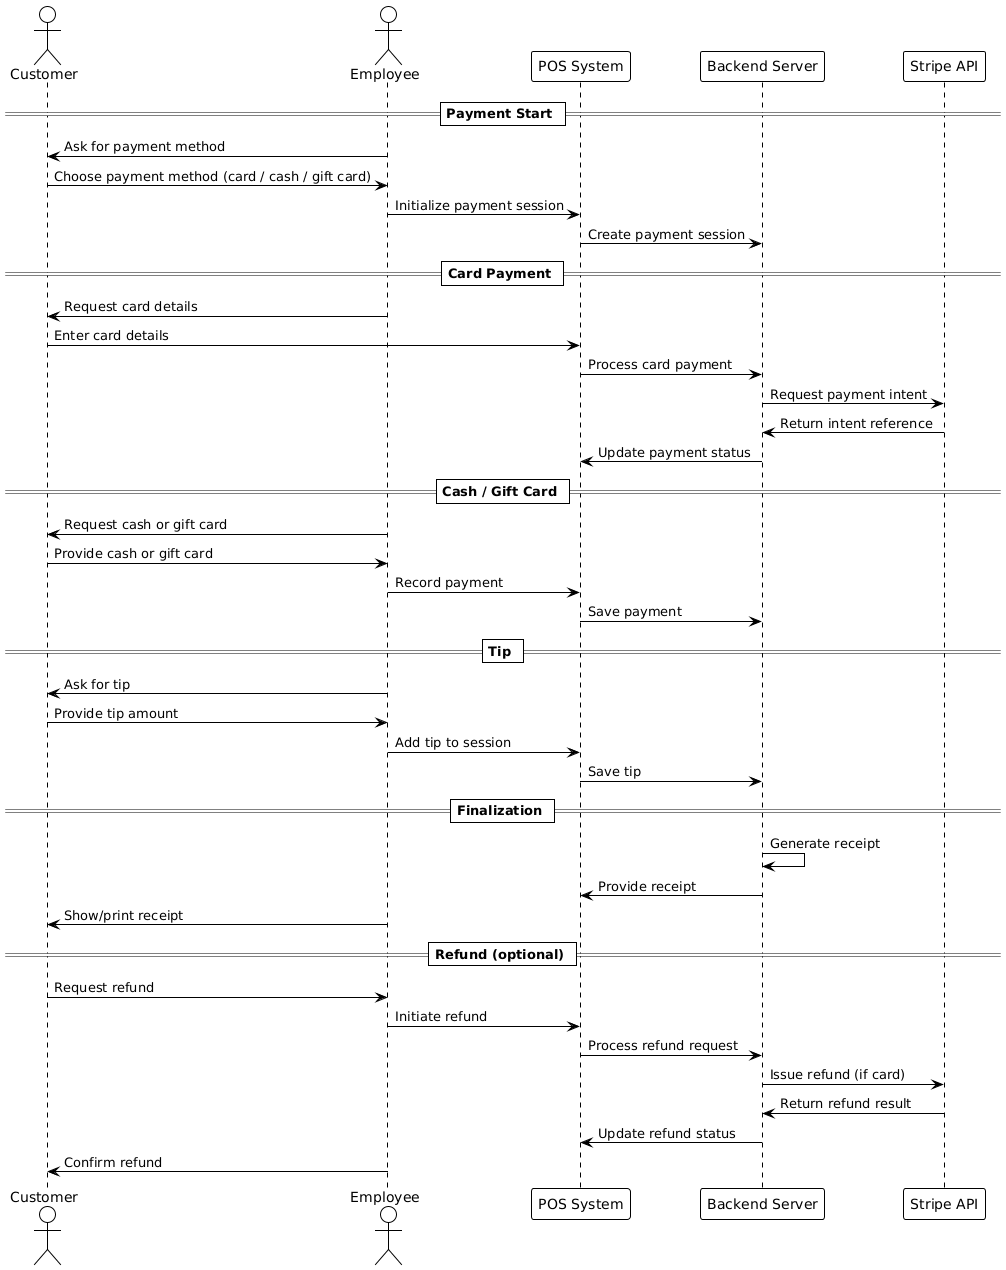
\includegraphics[width=0.95\textwidth]{images/diagrams/payment/payment_flow.png}
    \caption{Payment Flow Sequence Diagram}
    \label{fig:payment_flow}
\end{figure}

\subsection{Business Management}


% ------------------------------------------------------------------------
% MANAGEMENT DOMAIN (System-wide administrative and operational functions)
% ------------------------------------------------------------------------
% Use Case                           | Description
% ------------------------------------------------------------------------
% User Management                    | Specify business owner can only edit their business's users
% Manage Products/Services           | Add, edit, or deactivate products or services (e.g., menu items, massage types). 
% Manage Product Variations          | Create/edit modifiers for products (e.g., milk type, decaf, size)
% Manage Employees                   | Create, update, or deactivate employee accounts.
% Manage Business Info               | Update business details (owner, address, name, tax ID, contact info).
% Manage Inventory (Optional)        | Track stock levels of items (e.g., ingredients, products).
% Manage Taxes                       | Configure tax rates (e.g., VAT) for different products or services.
% Manage Users & Roles               | Assign permissions to employees (e.g., manager, cashier, admin).
% Super Admin Access                 | Special user (system operator) can access all businesses for support.
% View Reports                       | Generate reports on orders, appointments, revenue, etc.
% Manage Modifiers/Variants          | Define product variants (e.g., latte with almond milk, decaf).
% Manage Discounts                   | Create and manage discount rules (e.g., seasonal, loyalty).
% Manage Service Charges/Tips        | Manage Service Charges/Tips	Configure service charge/gratuity rules (change shouldn't affect historical records)
% Time-Limited Discounts             | Create discounts that are valid only for specific time periods
% ------------------------------------------------------------------------


% ------------------------------------------------------------------------
% Cross-Domain Use Cases (Apply to multiple domains)
% ------------------------------------------------------------------------
% | Use Case                 | Description                                             
% |--------------------------|---------------------------------------------------------
% | Login / Authentication   | Employees log into the system.                          
% | Logout                   | Secure session end.                                     
% | View History             | View past orders or appointments.                       
% | Historical Data Consistency Check   | Ensure changes (e.g., tax updates) don’t affect         
% |                                     | historical records.                                     
% ------------------------------------------------------------------------
We have identified the following Use cases for the Business management domain:

\vspace{1cm}
\begin{longtable}{p{0.25\linewidth} p{0.70\linewidth}}
\caption{Use cases for the Business Management domain} \\
\textbf{Use case} & \textbf{Description} \\
\hline
\endfirsthead

\multicolumn{2}{c}{{\tablename\ \thetable{} -- Continued from previous page}} \\
\textbf{Use case} & \textbf{Description} \\
\hline
\endhead

\multicolumn{2}{c}{{Continued on next page}} \\
\endfoot

\endlastfoot

User Management &
\begin{minipage}[t]{\linewidth}
The business owner can create, update, or deactivate users within their own business. They cannot modify accounts belonging to other businesses.
\end{minipage} \\[6pt]
\multicolumn{2}{@{}c@{}}{\color{gray}\rule{0.95\linewidth}{0.4pt}} \\[6pt]
Manage Employee Information &
\begin{minipage}[t]{\linewidth}
The Owner or Co-Owner views and modifies an employee’s information, performance, or feedback data.
\end{minipage} \\[6pt]
\multicolumn{2}{@{}c@{}}{\color{gray}\rule{0.95\linewidth}{0.4pt}} \\[6pt]
Manage Co-Owner Information &
\begin{minipage}[t]{\linewidth}
The Owner manages Co-Owners within the business. They can modify their permissions (e.g., access to employee management or financial data) or remove them entirely from the business.
\end{minipage} \\[6pt]
\multicolumn{2}{@{}c@{}}{\color{gray}\rule{0.95\linewidth}{0.4pt}} \\[6pt]
Manage Jobs &
\begin{minipage}[t]{\linewidth}
The owner or co-owner creates or modifies job roles for employees within a business. A job includes a name, description, assigned role, and an activity timetable specifying minimum and maximum durations for tasks.
\end{minipage} \\[6pt]
\multicolumn{2}{@{}c@{}}{\color{gray}\rule{0.95\linewidth}{0.4pt}} \\[6pt]
Manage Locations &
\begin{minipage}[t]{\linewidth}
The owner or co-owner manages business locations. A location includes address, open hours, and a seating plan represented as a grid with labeled tables (e.g., 2A, 5A, 1B). Locations can be created, modified, or deleted.
\end{minipage} \\[6pt]
\multicolumn{2}{@{}c@{}}{\color{gray}\rule{0.95\linewidth}{0.4pt}} \\[6pt]
Manage Businesses &
\begin{minipage}[t]{\linewidth}
The user views a list of their owned and co-owned businesses, opens a selected business to manage it, or creates a new one.
\end{minipage} \\[6pt]
\multicolumn{2}{@{}c@{}}{\color{gray}\rule{0.95\linewidth}{0.4pt}} \\[6pt]
Create or Edit Business &
\begin{minipage}[t]{\linewidth}
The user creates a new business by entering details such as name, description, type, specific type, and country, or edits an existing one through the business management view.
\end{minipage} \\[6pt]
\multicolumn{2}{@{}c@{}}{\color{gray}\rule{0.95\linewidth}{0.4pt}} \\[6pt]















% Manage Products \\ and Services &
% \begin{minipage}[t]{\linewidth}
% The business owner or authorized staff can add new products/services, edit details (name, price, category), or deactivate them (e.g., coffee, massage type).
% \end{minipage} \\[6pt]
% \multicolumn{2}{@{}c@{}}{\color{gray}\rule{0.95\linewidth}{0.4pt}} \\[6pt]
% Manage Product Variations &
% \begin{minipage}[t]{\linewidth}
% The business owner or staff can define or edit product modifiers, such as size (small/medium/large), add-ons or other options.
% \end{minipage} \\[6pt]
% \multicolumn{2}{@{}c@{}}{\color{gray}\rule{0.95\linewidth}{0.4pt}} \\[6pt]
% Manage Employees &
% \begin{minipage}[t]{\linewidth}
% The business owner can create new employee accounts, update employee details (role, contact, availability), or deactivate accounts.
% \end{minipage} \\[6pt]
% \multicolumn{2}{@{}c@{}}{\color{gray}\rule{0.95\linewidth}{0.4pt}} \\[6pt]
% Manage Business Info &
% \begin{minipage}[t]{\linewidth}
% The business owner can update business details such as the name, address, tax ID, contact information, or ownership information.
% \end{minipage} \\[6pt]
% \multicolumn{2}{@{}c@{}}{\color{gray}\rule{0.95\linewidth}{0.4pt}} \\[6pt]
% Manage Inventory (Optional) &
% \begin{minipage}[t]{\linewidth}
% The business can track and update stock levels of ingredients or products. System automatically reduces inventory when items are sold, and can alert when stock is low.
% \end{minipage} \\[6pt]
% \multicolumn{2}{@{}c@{}}{\color{gray}\rule{0.95\linewidth}{0.4pt}} \\[6pt]
% Manage Taxes &
% \begin{minipage}[t]{\linewidth}
% Admins can configure tax rules and rates (e.g., VAT, sales tax) for products or services. Updates affect only new transactions; historical data remains unchanged.
% \end{minipage} \\[6pt]
% \multicolumn{2}{@{}c@{}}{\color{gray}\rule{0.95\linewidth}{0.4pt}} \\[6pt]
% Manage Users \\ and Roles &
% \begin{minipage}[t]{\linewidth}
% The business owner can assign system roles (manager, cashier, admin, etc.) to employees, controlling access rights and permissions within the system.
% \end{minipage} \\[6pt]
% \multicolumn{2}{@{}c@{}}{\color{gray}\rule{0.95\linewidth}{0.4pt}} \\[6pt]
% Super Admin Access &
% \begin{minipage}[t]{\linewidth}
% A system operator (Super Admin) can access any business account in the system for technical support, troubleshooting, or emergency fixes.
% \end{minipage} \\[6pt]
% \multicolumn{2}{@{}c@{}}{\color{gray}\rule{0.95\linewidth}{0.4pt}} \\[6pt]
% Manage Modifiers/Variants &
% \begin{minipage}[t]{\linewidth}
% Admin can define product variants such as “latte with almond milk” or “spa service with aromatherapy add-on.” Variants allow customer customization at order time.
% \end{minipage} \\[6pt]
% \multicolumn{2}{@{}c@{}}{\color{gray}\rule{0.95\linewidth}{0.4pt}} \\[6pt]
% Manage Discounts &
% \begin{minipage}[t]{\linewidth}
% Admins can create and manage discount rules (percentage-based, fixed amount, seasonal campaigns, loyalty discounts).
% \end{minipage} \\[6pt]
% \multicolumn{2}{@{}c@{}}{\color{gray}\rule{0.95\linewidth}{0.4pt}} \\[6pt]
% Manage Service Charges/Tips &
% \begin{minipage}[t]{\linewidth}
% Admins can configure rules for applying service charges or gratuities. Updates only apply to future transactions, ensuring historical data remains intact.
% \end{minipage} \\[6pt]
% \multicolumn{2}{@{}c@{}}{\color{gray}\rule{0.95\linewidth}{0.4pt}} \\[6pt]
% Time-Limited Discounts &
% \begin{minipage}[t]{\linewidth}
% Admins can create discounts restricted to a specific timeframe (e.g., happy hour, seasonal promotions). The system enforces validity automatically.
% \end{minipage} \\[6pt]
% \multicolumn{2}{@{}c@{}}{\color{gray}\rule{0.95\linewidth}{0.4pt}} \\[6pt]

\end{longtable}






We have identified the following Cross-Domain Use cases for the Business management domain:
\vspace{1cm}
\begin{longtable}{p{0.25\linewidth} p{0.70\linewidth}}
\caption{Cross-Domain Use cases for the Business Management domain} \\
\textbf{Use case} & \textbf{Description} \\
\hline
\endfirsthead

\multicolumn{2}{c}{{\tablename\ \thetable{} -- Continued from previous page}} \\
\textbf{Use case} & \textbf{Description} \\
\hline
\endhead

\multicolumn{2}{c}{{Continued on next page}} \\
\endfoot

\endlastfoot

Login / Authentication &
\begin{minipage}[t]{\linewidth}
Employees log into the system using their credentials. The system validates identity and assigns permissions based on role.
\end{minipage} \\[6pt]
\multicolumn{2}{@{}c@{}}{\color{gray}\rule{0.95\linewidth}{0.4pt}} \\[6pt]
Logout &
\begin{minipage}[t]{\linewidth}
Employees securely end their session. The system clears active tokens/sessions and confirms logout Users (customers, employees, or admins) can view past orders, appointments, or reports. This ensures transparency and auditability.
\end{minipage} \\[6pt]
\multicolumn{2}{@{}c@{}}{\color{gray}\rule{0.95\linewidth}{0.4pt}} \\[6pt]
% View Historical Data, Consistency Check &
% \begin{minipage}[t]{\linewidth}
% Users (customers, employees, or admins) can view past orders, appointments, or reports. This ensures transparency and auditability.
% \end{minipage} \\[6pt]
% \multicolumn{2}{@{}c@{}}{\color{gray}\rule{0.95\linewidth}{0.4pt}} \\[6pt]
% Historical Data Consistency Check &
% \begin{minipage}[t]{\linewidth}
% The system ensures that administrative changes (tax rates, discounts, service charges) apply only to new transactions, without modifying historical order or appointment records.
% \end{minipage} \\[6pt]
% \multicolumn{2}{@{}c@{}}{\color{gray}\rule{0.95\linewidth}{0.4pt}} \\[6pt]

\end{longtable}
% related use cases: User Management, Manage Employees, Manage Users & Roles, Super Admin Access

\newpage
\subsubsection{User Management Business Flow}

\begin{center}
\setlength{\tabcolsep}{8pt}
\renewcommand{\arraystretch}{1.3}
\begin{tabular}{|p{0.48\linewidth}|p{0.48\linewidth}|}
\hline
\textbf{Tables / Entities} \newline
\begin{mpitemlist}
\item \textbf{Owner} – represents the business owner managing users.
\item \textbf{User} – represents employees or co-owners tied to a business.
\item \textbf{Business} – links users to the correct business context.
\item \textbf{User Table} – stores all user data, including roles, status, and associations.
\item \textbf{Auth Session} – identifies and validates logged-in users and their permissions.
\end{mpitemlist}
&
\textbf{Components} \newline
\begin{mpitemlist}
\item \textbf{User Interface} – pages and forms for inviting, generating codes, searching, and managing users.
\item \textbf{Auth Service} – validates ownership and permissions for each action.
\item \textbf{User Service} – executes create, update, and deactivate logic.
\item \textbf{Database Layer} – persists and retrieves user data.
\end{mpitemlist}
\\ \hline
\textbf{User Actions} \newline
\begin{mpitemlist}
\item Log in to the system.
\item Navigate to \textit{Business → Specific Business → Employees}.
\item Choose between inviting, generating code, or managing existing employees.
\item Fill in forms or search employee records.
\item Confirm actions and receive immediate feedback.
\end{mpitemlist}
&
\textbf{System Reactions} \newline
\begin{mpitemlist}
\item Validate the user’s permissions and business ownership via the Auth Service.
\item Execute the requested operation through the User Service.
\item Commit changes to the database.
\item Return operation result to the UI (toast messages or errors).
\end{mpitemlist}
\\ \hline
\end{tabular}
\end{center}


\begin{figure}[H]
    \centering
    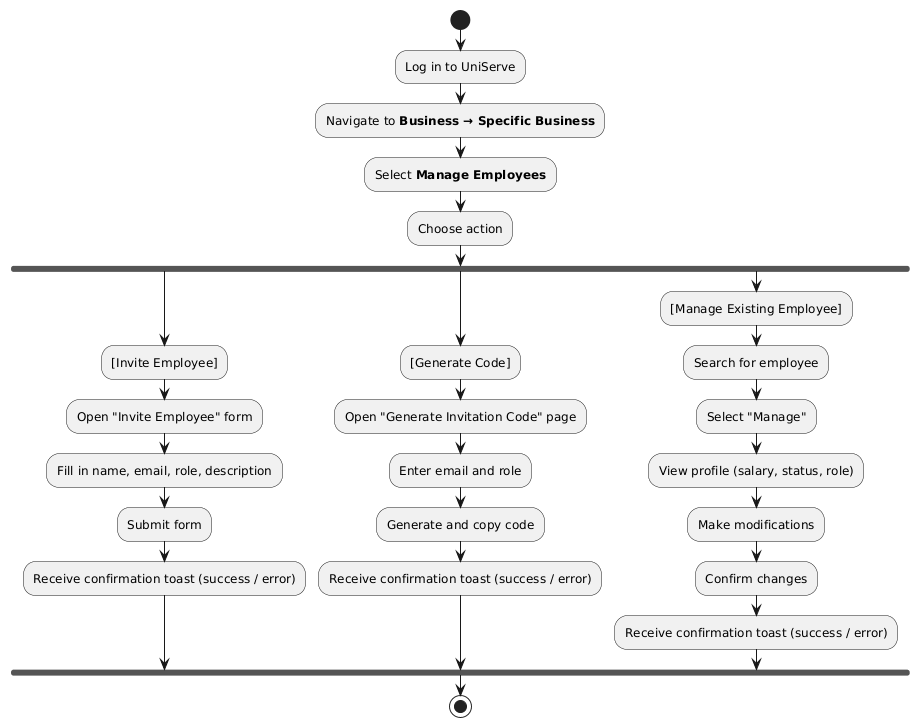
\includegraphics[width=1\textwidth]{docs/ps-design/design-document/images/diagrams/business/bpmn_user_manage.png}
    \caption{Employee Management Business Flow Diagram}
    \label{fig:user_manage_flow}
\end{figure}
\begin{figure}[H]
    \centering
    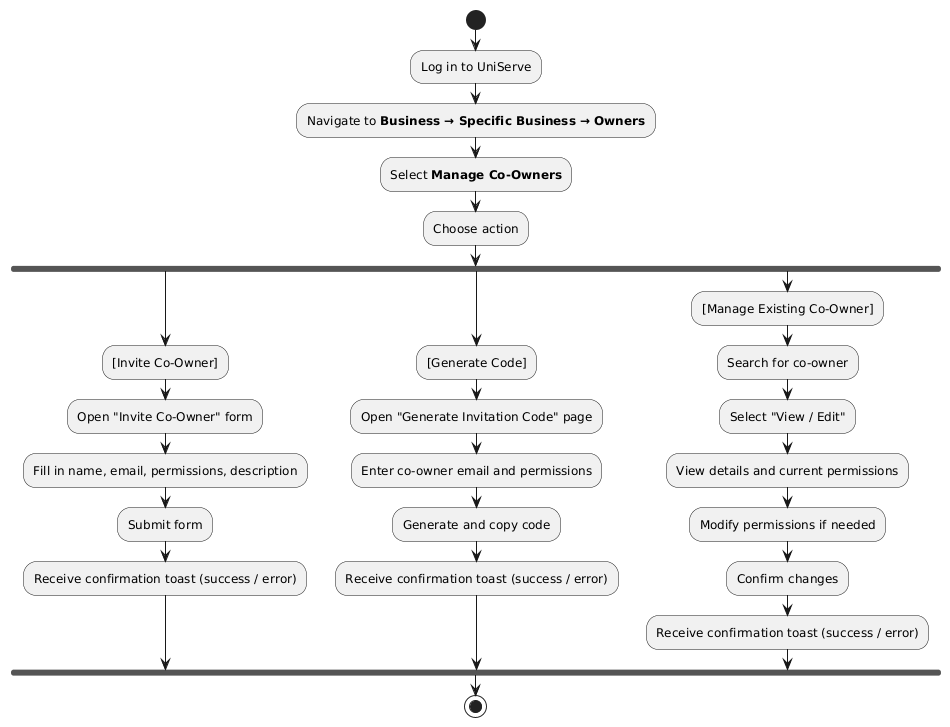
\includegraphics[width=1\textwidth]{docs/ps-design/design-document/images/diagrams/business/bpmn_user_manage_coowner.png}
    \caption{Co-Owner Management Business Flow Diagram}
    \label{fig:user_manage_flow}
\end{figure}

\subsubsection{Manage Employee Information Business Flow}
\begin{center}
\setlength{\tabcolsep}{8pt}
\renewcommand{\arraystretch}{1.3}
\begin{tabular}{|p{0.48\linewidth}|p{0.48\linewidth}|}
\hline
\textbf{Tables / Entities} \newline
\begin{mpitemlist}
\item \textbf{Owner / Co-Owner} – represents the business management roles responsible for viewing or modifying employee data.
\item \textbf{Employee} – represents staff members whose data, performance, and feedback are being managed.
\item \textbf{Business} – links employees to the correct business context under which they operate.
\item \textbf{Employee Table} – stores information about salary, position, work hours, and employment status.
\item \textbf{Performance Data} – tracks employee task completion and inventory changes.
\item \textbf{Feedback Data} – stores ratings and written feedback given by managers or coworkers.
\end{mpitemlist}
&
\textbf{Components} \newline
\begin{mpitemlist}
\item \textbf{Employee Management UI} – interface for viewing, modifying, and navigating employee information, performance, and feedback pages.
\item \textbf{Auth Service} – validates access permissions for Owners and Co-Owners.
\item \textbf{Employee Service} – handles data retrieval, modification, and validation of employee details.
\item \textbf{Analytics Service} – retrieves and aggregates employee performance metrics.
\item \textbf{Feedback Service} – fetches ratings and written reviews related to the employee.
\item \textbf{Database Layer} – stores and retrieves all related employee, performance, and feedback records.
\end{mpitemlist}
\\ \hline
\textbf{User Actions} \newline
\begin{mpitemlist}
\item Log in to the system.
\item Navigate to \textit{Business → Employees}.
\item Select \textit{Manage Employee} and search for a specific employee.
\item Choose one of the following actions:
    \begin{itemize}
        \item Modify Information (update salary, hours, or employment status)
        \item View Performance (inspect graphs and metrics)
        \item View Feedback (read and filter ratings and reviews)
    \end{itemize}
\item Save any modifications and confirm the changes.
\end{mpitemlist}
&
\textbf{System Reactions} \newline
\begin{mpitemlist}
\item Authenticate and verify that the user has permission to manage the employee.
\item Load and display the selected employee’s data.
\item Execute updates or retrieve requested information through the respective services.
\item Persist modifications in the database.
\item Return a visual confirmation (toast message) or error if the operation fails.
\item Refresh the employee profile view with updated data.
\end{mpitemlist}
\\ \hline
\end{tabular}
\end{center}
\begin{figure}[H]
    \centering
    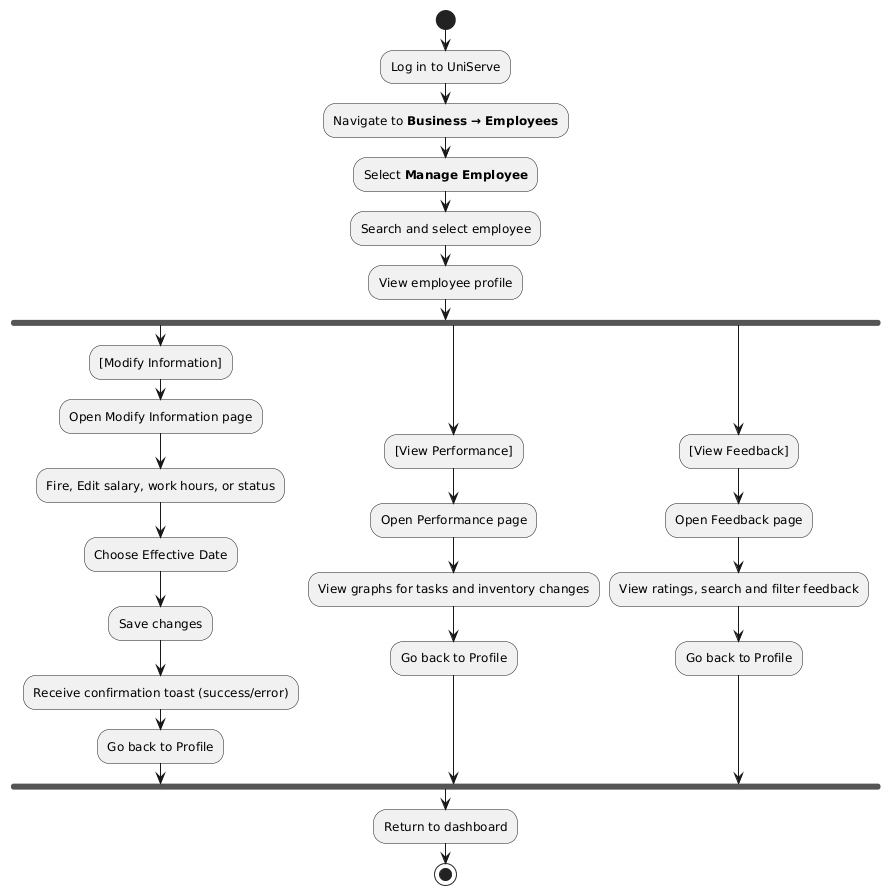
\includegraphics[width=1\textwidth]{docs/ps-design/design-document/images/diagrams/business/bpmn_manage_employee.png}
    \caption{Employee Information Management Business Flow Diagram}
    \label{fig:user_manage_flow}
\end{figure}

\subsubsection{Manage Co-Owner Information Business Flow}

\begin{center}
\setlength{\tabcolsep}{8pt}
\renewcommand{\arraystretch}{1.3}
\begin{tabular}{|p{0.48\linewidth}|p{0.48\linewidth}|}
\hline
\textbf{Tables / Entities} \newline
\begin{mpitemlist}
\item \textbf{Owner} – represents the business owner with full control over co-owner management.
\item \textbf{Co-Owner} – represents a secondary manager with assigned permissions.
\item \textbf{Business} – links co-owners and permissions to the corresponding business.
\item \textbf{Permissions Table} – defines access levels such as managing employees or viewing finances.
\item \textbf{Auth Session} – authenticates the logged-in Owner and verifies access control.
\end{mpitemlist}
&
\textbf{Components} \newline
\begin{mpitemlist}
\item \textbf{Owner Management UI} – interface for selecting, editing, or removing co-owners.
\item \textbf{Auth Service} – validates the Owner’s authority and permission scopes.
\item \textbf{Co-Owner Service} – processes permission updates and removal operations.
\item \textbf{Database Layer} – stores relationships between Owners, Co-Owners, and assigned permissions.
\item \textbf{Notification System} – provides success or error feedback to the user.
\end{mpitemlist}
\\ \hline
\textbf{User Actions} \newline
\begin{mpitemlist}
\item Log in to UniServe.
\item Navigate to \textit{Business → Owners}.
\item Select a Co-Owner from the list.
\item Choose to \textit{Modify Permissions} or \textit{Remove from Business}.
\item If modifying, toggle permissions and click \textit{Save}.
\item Confirm any removal actions.
\item Return to the Owners list or dashboard.
\end{mpitemlist}
&
\textbf{System Reactions} \newline
\begin{mpitemlist}
\item Validate Owner authorization through the Auth Service.
\item Load selected Co-Owner data and associated permissions.
\item Apply updates or execute removal through the Co-Owner Service.
\item Commit changes to the database.
\item Display confirmation or error toast message.
\item Update the interface with the current state of Co-Owners.
\end{mpitemlist}
\\ \hline
\end{tabular}
\end{center}

\begin{figure}[H]
    \centering
    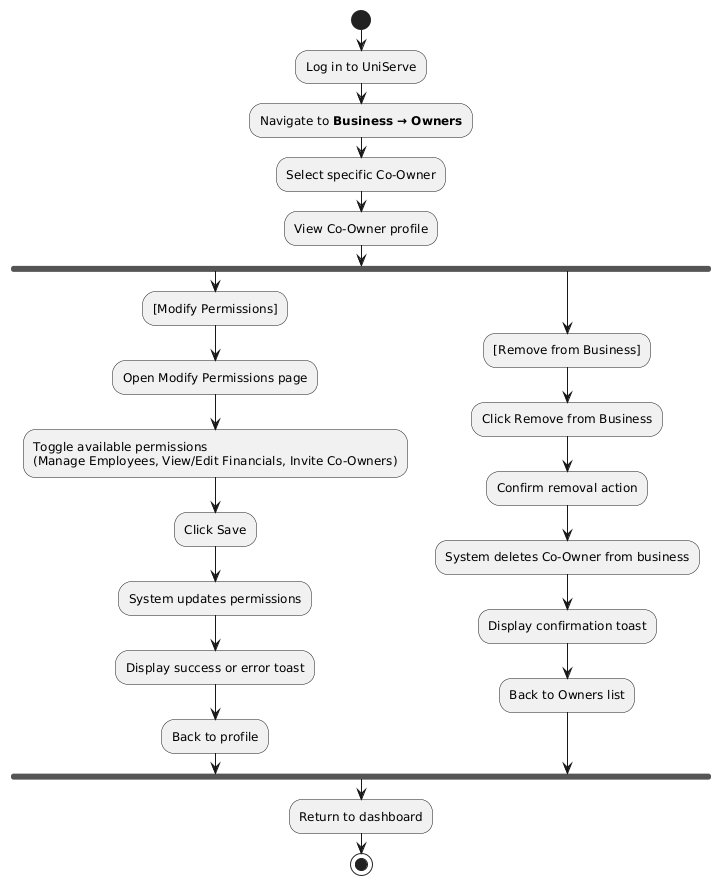
\includegraphics[width=0.6\textwidth]{docs/ps-design/design-document/images/diagrams/business/bpmn_manage_coowner_information.png}
    \caption{Co-Owner Information Management Business Flow Diagram}
    \label{fig:manage_co_owner_information_business_flow}
\end{figure}

\subsubsection{Manage Jobs Business Flow}
\begin{center}
\setlength{\tabcolsep}{8pt}
\renewcommand{\arraystretch}{1.3}
\begin{tabular}{|p{0.48\linewidth}|p{0.48\linewidth}|}
\hline
\textbf{Tables / Entities} \newline
\begin{mpitemlist}
\item \textbf{Business} – represents the company owning job definitions.
\item \textbf{Job} – stores job metadata such as name, description, and associated role.
\item \textbf{Timetable} – defines activity steps with minimum and maximum durations.
\item \textbf{User} – owner or co-owner managing job entries.
\end{mpitemlist}
&
\textbf{Components} \newline
\begin{mpitemlist}
\item \textbf{Job Management UI} – interface for creating or editing job details.
\item \textbf{Job Service} – handles creation, validation, and updates of job data.
\item \textbf{Timetable Manager} – manages per-job activity scheduling.
\item \textbf{Auth Service} – checks user permission to manage jobs.
\item \textbf{Database Layer} – persists job and timetable entities.
\end{mpitemlist}
\\ \hline
\textbf{User Actions} \newline
\begin{mpitemlist}
\item Navigate to “Jobs”.
\item Create or edit a job.
\item Fill in details and add timetable activities.
\item Save the job.
\end{mpitemlist}
&
\textbf{System Reactions} \newline
\begin{mpitemlist}
\item Validate form data.
\item Persist or update job records.
\item Display feedback to user (success or error).
\item Refresh job list view.
\end{mpitemlist}
\\ \hline
\end{tabular}
\end{center}
\begin{figure}[H]
    \centering
    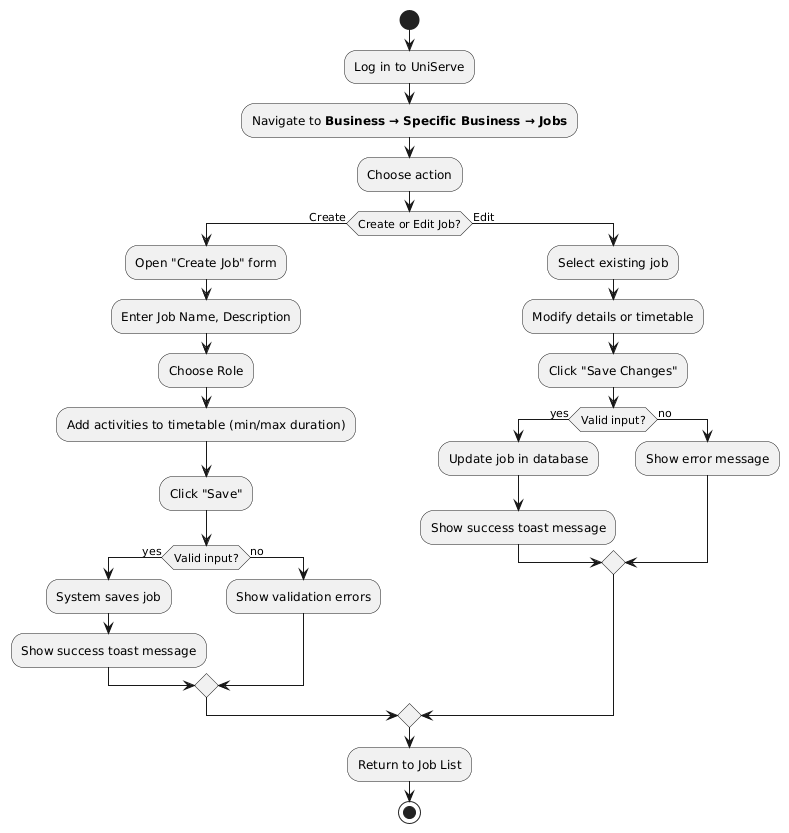
\includegraphics[width=0.6\textwidth]{docs/ps-design/design-document/images/diagrams/business/bpmn_manage_jobs.png}
    \caption{Job Management Business Flow Diagram}
    \label{fig:manage_jobs_business_flow}
\end{figure}

\subsubsection{Manage Locations Business Flow}
\begin{center}
\setlength{\tabcolsep}{8pt}
\renewcommand{\arraystretch}{1.3}
\begin{tabular}{|p{0.48\linewidth}|p{0.48\linewidth}|}
\hline
\textbf{Tables / Entities} \newline
\begin{mpitemlist}
\item \textbf{Business} – represents the company managing multiple branches or locations.
\item \textbf{Location} – stores name, address, and operating details.
\item \textbf{Seating Plan} – defines the layout of tables in a grid format (e.g., 2A, 1B).
\item \textbf{User} – owner or co-owner who manages locations.
\end{mpitemlist}
&
\textbf{Components} \newline
\begin{mpitemlist}
\item \textbf{Location Management UI} – interface for creating, editing, or deleting locations.
\item \textbf{Seating Plan Editor} – grid editor for table positioning.
\item \textbf{Location Service} – handles creation, updates, and deletion of location records.
\item \textbf{Auth Service} – ensures only authorized users can manage locations.
\item \textbf{Database Layer} – persists location and seating plan data.
\end{mpitemlist}
\\ \hline
\textbf{User Actions} \newline
\begin{mpitemlist}
\item Navigate to “Locations”.
\item Add, edit, or delete a location.
\item Input name, address, hours, and seating plan.
\item Save or confirm deletion.
\end{mpitemlist}
&
\textbf{System Reactions} \newline
\begin{mpitemlist}
\item Validate and persist data.
\item Update or remove location records.
\item Show success or error message.
\item Refresh the list of locations.
\end{mpitemlist}
\\ \hline
\end{tabular}
\end{center}
\begin{figure}[H]
    \centering
    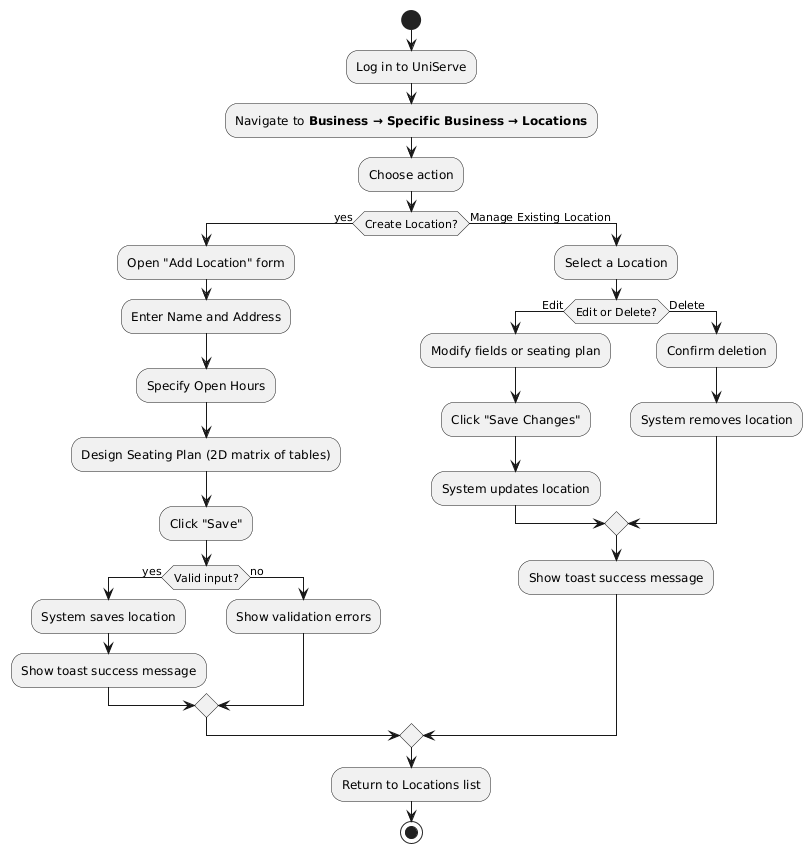
\includegraphics[width=0.6\textwidth]{docs/ps-design/design-document/images/diagrams/business/bpmn_manage_locations.png}
    \caption{Location Management Business Flow Diagram}
    \label{fig:manage_locations_business_flow}
\end{figure}

\subsubsection{Manage Businesses Business Flow}
\begin{center}
\setlength{\tabcolsep}{8pt}
\renewcommand{\arraystretch}{1.3}
\begin{tabular}{|p{0.48\linewidth}|p{0.48\linewidth}|}
\hline
\textbf{Tables / Entities} \newline
\begin{mpitemlist}
\item \textbf{User} – represents the logged-in person.
\item \textbf{Business} – contains business details such as name, description, type, and country.
\end{mpitemlist}
&
\textbf{Components} \newline
\begin{mpitemlist}
\item \textbf{Business Management UI} – displays owned and co-owned businesses.
\item \textbf{Business Service} – fetches user-related businesses from the database.
\item \textbf{Navigation Controller} – handles transitions to business management or creation views.
\end{mpitemlist}
\\ \hline
\textbf{User Actions} \newline
\begin{mpitemlist}
\item View list of owned and co-owned businesses.
\item Open a specific business.
\item Create a new business.
\end{mpitemlist}
&
\textbf{System Reactions} \newline
\begin{mpitemlist}
\item Retrieve business list from backend.
\item Display businesses with open buttons.
\item Redirect to business creation or details view.
\end{mpitemlist}
\\ \hline
\end{tabular}
\end{center}

\begin{figure}[H]
    \centering
    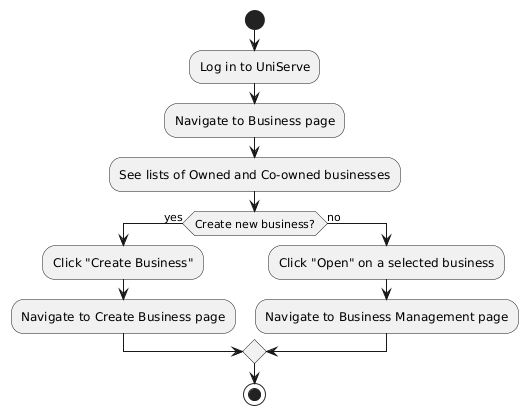
\includegraphics[width=0.6\textwidth]{docs/ps-design/design-document/images/diagrams/business/bpmn_manage_businesses.png}
    \caption{Manage Businesses Business Flow Diagram}
    \label{fig:manage_businesses_flow}
\end{figure}
\subsubsection{Create or Edit Business Flow}
\begin{center}
\setlength{\tabcolsep}{8pt}
\renewcommand{\arraystretch}{1.3}
\begin{tabular}{|p{0.48\linewidth}|p{0.48\linewidth}|}
\hline
\textbf{Tables / Entities} \newline
\begin{mpitemlist}
\item \textbf{Business} – stores business metadata such as name, description, type, specific type, and country.
\item \textbf{User} – the creator or editor of the business.
\end{mpitemlist}
&
\textbf{Components} \newline
\begin{mpitemlist}
\item \textbf{Business Creation UI} – form for entering and editing business details.
\item \textbf{Business Service} – validates and persists business data.
\item \textbf{Auth Service} – checks that user has permission to create or edit businesses.
\item \textbf{Database Layer} – saves or updates business records.
\end{mpitemlist}
\\ \hline
\textbf{User Actions} \newline
\begin{mpitemlist}
\item Fill in name, description, and type.
\item Choose specific type and country.
\item Create or save changes.
\end{mpitemlist}
&
\textbf{System Reactions} \newline
\begin{mpitemlist}
\item Validate input fields.
\item Persist new or updated business data.
\item Show feedback to user.
\item Redirect to Manage Businesses page.
\end{mpitemlist}
\\ \hline
\end{tabular}
\end{center}

\begin{figure}[H]
    \centering
    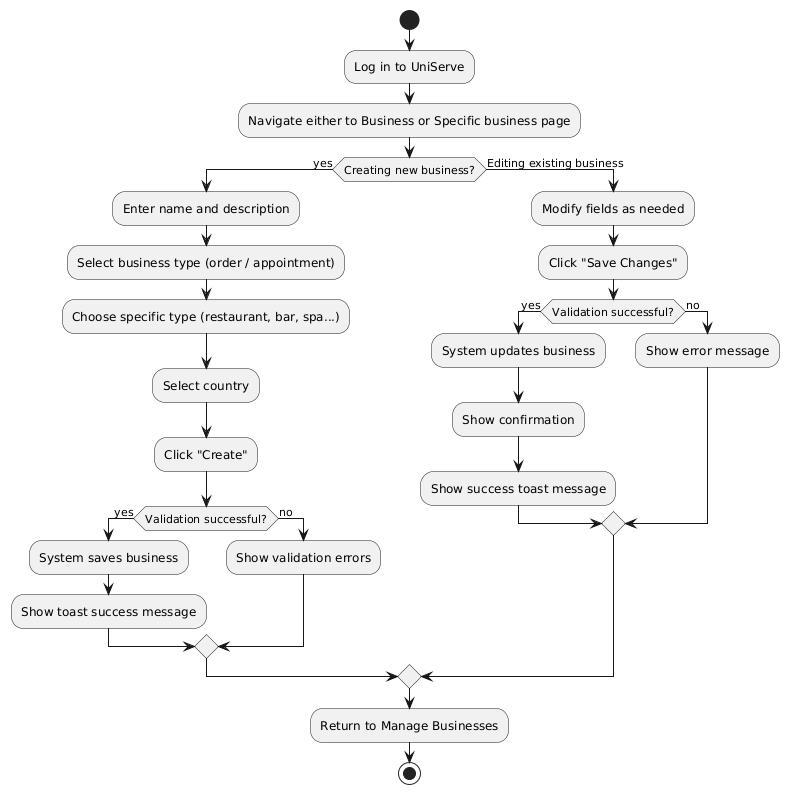
\includegraphics[width=0.6\textwidth]{docs/ps-design/design-document/images/diagrams/business/bpmn_manage_business_information.png}
    \caption{Create or Edit Business Business Flow Diagram}
    \label{fig:manage_businesses_flow}
\end{figure}



\section{APIs}

Present as an openapi.yaml file. PR: \url{https://github.com/user5427/ps-design/pull/7}

% \todocomment{Sort/filter/pagination. Decide on the details and add to the yaml.}

% \todocomment{Auth: currently uses JWT access tokens. Write in here why we chose this approach, the pros/cons and possible alternatives.}

For authentication, we selected a stateless strategy using JSON Web Tokens (JWT). Statelessness is ideal for scaling our decoupled frontend and backend APIs without complex session management. While a powerful identity provider like Keycloak was considered, it was deferred due to its significant infrastructure and implementation complexity. JWT offers the best balance of scalability and simplicity for the project's current scope.




% \section{Data Model}

% \yellowcomment{better to specify in each order/service/managing/and other functionality domain separately}

% \subsection{Order Data Model}
% \begin{figure}[H]
%     \centering
%     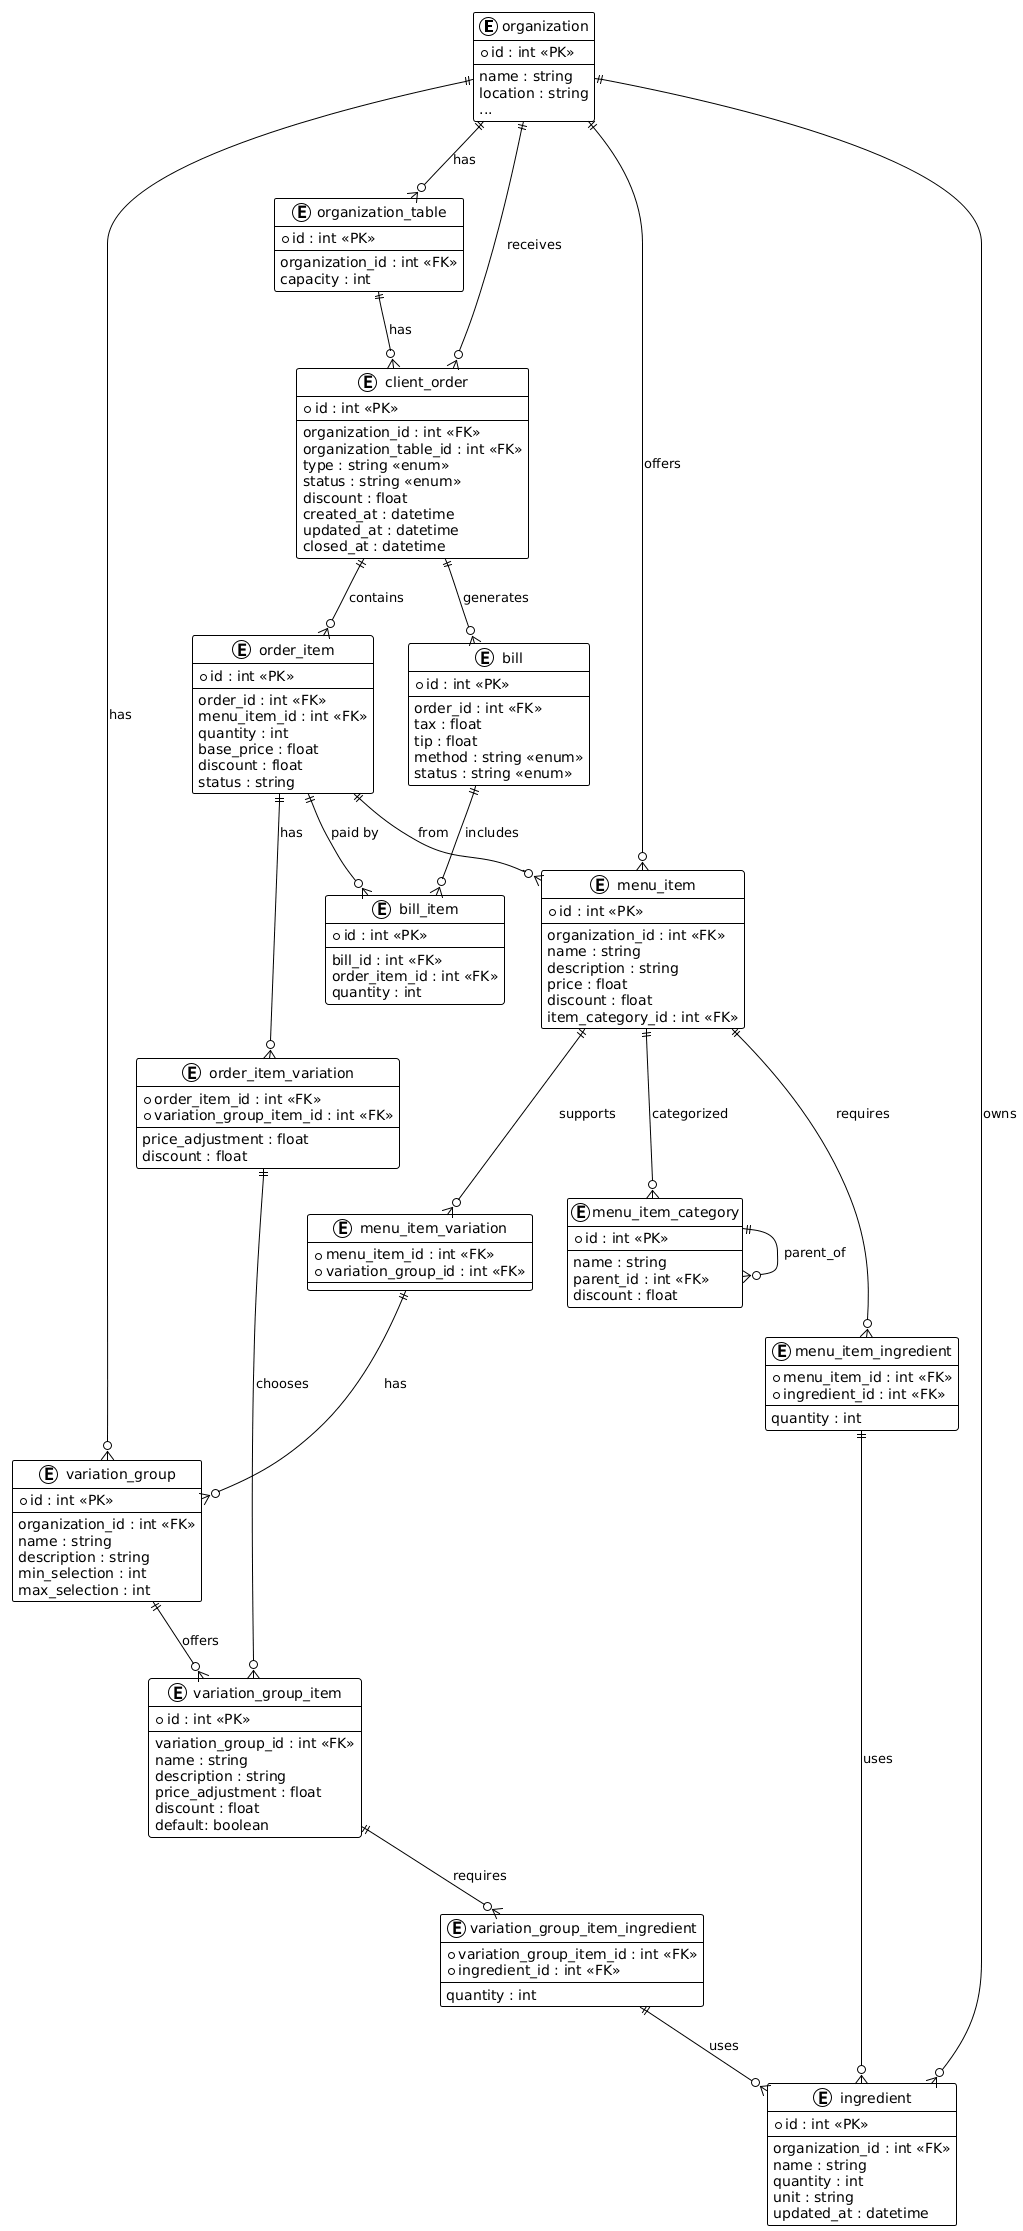
\includegraphics[width=0.65\textwidth]{images/diagrams/orders/order_model_class.png}
%     \caption{Order Class Diagram}
%     \label{fig:order_class_diagram}
% \end{figure}

% \subsection{Service Data Model}

% \subsection{Business Data Model}

% \subsubsection{Design Decisions (Summary)}

% Below are the initial data design decisions for business and user account management. 
% \begin{itemize}
%     \item \textbf{User role-based access control (RBAC):} Roles group permissions, and users are assigned to roles. Also allow per-business role assignment.
%     \item \textbf{Identifiers and timestamps:} Use UUID primary keys and maintain \texttt{created} and \texttt{updated\_at} timestamps. This supports managing multiple businesses, potentially distributed across systems.
%     \item \textbf{Password security:} Store only hashed passwords. Include fields \texttt{password\_hash}, \texttt{password\_algo/version}, and \texttt{password\_changed\_at}. Do not store plaintext passwords or use reversible encryption.
%     \item \textbf{Audit logging:} Track login attempts, password resets, and administrator or manager actions.
%     \item \textbf{Support sessions or tokens:} Either server-side session store or JWT approach.
%     \item \textbf{Soft-delete:} For users with \textbf{is\_active} and \textbf{deleted\_at} attributes.
% \end{itemize}
% \textit{RBAC = Role-Based Access Control}

% \subsubsection{Entities and Tables}  

% The database schema is organized into the following entities and supporting tables:  

% \begin{itemize}
%     \item \textbf{organization}  
%     \begin{itemize}
%         \item id (PK), name, metadata, created\_at, updated\_at
%     \end{itemize}
%     \item \textbf{businesses}  
%     \begin{itemize}
%         \item id (PK), organization\_id (FK), name, metadata, created\_at, updated\_at
%     \end{itemize}
%     \item \textbf{users}  
%     \begin{itemize}
%         \item id (PK), organization\_id (FK), business\_id (FK, optional), email, display\_name, username, 
%         password\_hash, password\_algo, password\_version, is\_active, email\_verified, last\_login\_at, 
%         failed\_login\_attempts, locked\_until, created\_at, updated\_at
%     \end{itemize}
%     \item \textbf{roles}  
%     \begin{itemize}
%         \item id (PK), name, description, created\_at
%     \end{itemize}
%     \item \textbf{permissions}  
%     \begin{itemize}
%         \item id (PK), name, description
%     \end{itemize}
%     \item \textbf{role\_permissions}  
%     \begin{itemize}
%         \item role\_id (FK), permission\_id (FK)
%     \end{itemize}
%     \item \textbf{user\_roles}  
%     \begin{itemize}
%         \item user\_id (FK), role\_id (FK), assigned\_by (FK), assigned\_at
%     \end{itemize}
%     \item \textbf{user\_business\_roles}  
%     \begin{itemize}
%         \item user\_id (FK), business\_id (FK), role\_id (FK), assigned\_by (FK), assigned\_at
%     \end{itemize}
%     \item \textbf{sessions}  
%     \begin{itemize}
%         \item id (PK), user\_id (FK), session\_token, user\_agent, ip, created\_at, last\_seen\_at, expires\_at, revoked
%     \end{itemize}
%     \item \textbf{password\_resets}  
%     \begin{itemize}
%         \item id (PK), user\_id (FK), reset\_token, expires\_at, used\_at
%     \end{itemize}
%     \item \textbf{audit\_logs}  
%     \begin{itemize}
%         \item id (PK), user\_id (subject, FK), actor\_id (FK), action, resource\_type, resource\_id, details, created\_at
%     \end{itemize}
% \end{itemize}

% \textit{PK = Primary Key,}
% \textit{FK = Foreign Key}

% \subsubsection{Relationships}

% Below are the relationships between tables and entities in this schema.
% \begin{itemize}
%     \item \textbf{Organization $\rightarrow$ Businesses}. One organization can own many businesses. This models a parent company with multiple branches.
%     \item \textbf{Organization $\rightarrow$ Users}. One organization can have many users. Users are scoped to an organization.
%     \item \textbf{Businesses $\rightarrow$ Users (Optional)}. Users may also have a default \textbf{business\_id} to the business if are tied to one. But users don't have to be tied to a single business. They might be org-level (super admin or a lead manager).
%     \item \textbf{Businesses $\rightarrow$ User Store Roles}. A business can have many \textbf{user\_store\_roles}. This lets the assignment of roles to specific businesses.
%     \item \textbf{Users $\rightarrow$ Sessions}. One user can have many sessions (logins). Tracks IPs, session tokens, devices.
%     \item \textbf{Users $\rightarrow$ User Roles (Organization-wide)}. A user can have many roles at the organization level.
%     \item \textbf{Users $\rightarrow$ User Business Roles}. A user can have different roles in different businesses.
%     \item \textbf{Users $\rightarrow$ Audit Logs}. A user can generate many audit log entries as an actor. A user can also be the subject of audit logs.
%     \item \textbf{Roles $\rightarrow$ Role Permissions}. One role can have many permissions.
%     \item \textbf{Permissions $\rightarrow$ Role Permissions}. One permission can belong to many roles.
%     \item \textbf{Roles $\rightarrow$ User Roles}. A role can be assigned to many users throughout the organization.
%     \item \textbf{Roles $\rightarrow$ User Business Roles}. A role can be assigned to many users within a specific business.
% \end{itemize}

% \begin{figure}[H]
%     \centering
%     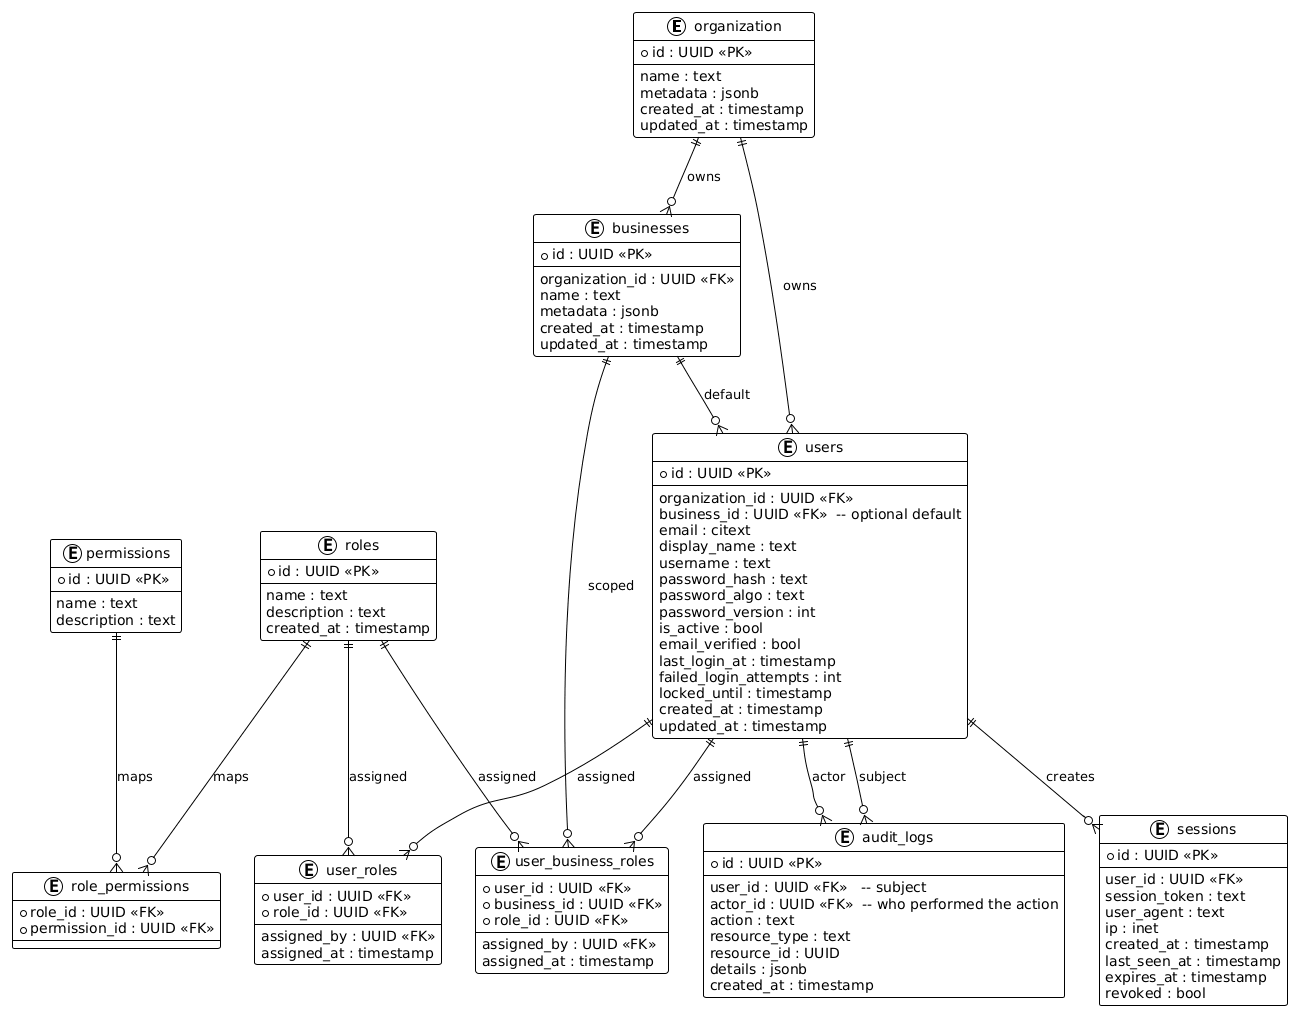
\includegraphics[width=0.8\textwidth]{images/diagrams/business/data_model_business.png}
%     \caption{Business Class Diagram with Attributes}
%     \label{fig:business_class_diagram}
% \end{figure}
% This diagram represents different relationships between different entities as well as their attributes. 

% \printbibliography[title = {References and sources}]

\end{document}
